\chapter{Background}

In this chapter, the mechanical design and kinematic relationships of the surgical robot developed in the iRAMs! project will be reviewed. The Jacobian matrix and the Jacobian pseudoinverse approach are presented as an iterative solution to the inverse kinematics problem. Lastly, there is a short introduction to the V-REP simulation environment and the Dampened Least Squares method used by V-REPs internal inverse kinematics solver. 

\section{Mechanical Design}
\begin{figure}[b!]
	\begin{center}
		%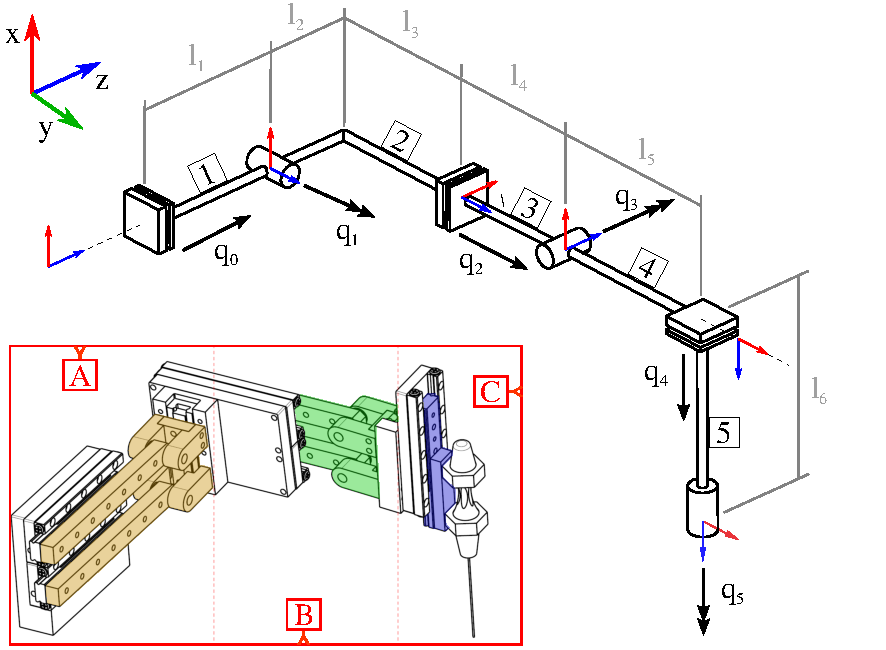
\includegraphics[width=15cm]{manipulator_overview_refactored}
		\import{images/}{manipulator_overview_refactored_tex.pdf_tex}
		\caption{The simplified serial manipulator, consisting of two subsequent PCJM elements (A and B) and a simple prismatic stage (C). Each PCJM element can be modelled as a translation and a following rotation. Adapted from \cite{Master_thesis}.}
		\label{Manipulator}
	\end{center}
\end{figure}

The surgical robot considered in this thesis consists of two subsequent \textit{Parallel Coupled Joint Mechanisms} (PCJMs), one single prismatic joint and one optional revolute joint, providing six degrees of freedom.

Each PCJM consists of two stick-slip piezo actuators moving parallel to each other at a distance \textit{d}. 
Translating both sliders the same distance results in a pure translation of the manipulator, while a differential movement results in an additional rotation. In contrast to a linear chain of prismatic and revolute joints, the PCJM approach provides higher stiffness and precision. 

\begin{figure}[t!]
	%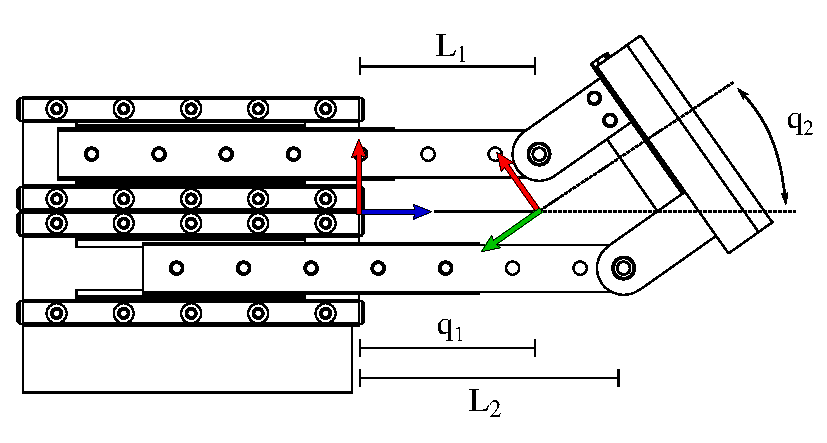
\includegraphics[width=\textwidth]{pcjm}
	\import{images/}{pcjm_refactored_tex.pdf_tex}
	\caption{A single Parallel Coupled Joint Mechanism. Differential displacement of the two prismatic joints $L_1$ and $L_2$ results in both a translation and rotation of the subsequent link. Adapted from \cite{Ali_FK}.}
	\label{pcjm}
\end{figure}

For a simpler kinematic analysis, the PCJM elements can be treated as a prismatic and subsequent revolute joint.
The two translations $L_1$ and $L_2$ correspond to the translation of the prismatic joint $q_0$ and angle of the revolute joint $q_1$ as
\begin{eqnarray}
	q_0	&=&	\frac{L_1+L_2}{2} \\
	q_1	&=&	\arctan(\frac{L_2-L_1}{d})\;.
\end{eqnarray}

Conversely, given the two joint positions $q_0$ and $q_1$, the slider positions can be uniquely determined via: 
\begin{eqnarray}
	L_1	&=&	\frac{d\cdot \tan(q_1)}{2}+q_0 \\
	L_2	&=& 2 q_0-L_1\;.
\end{eqnarray}


\section{Forward Kinematics}\label{FK}

In order to describe the position of the end effector relative to the base coordinate frame we determine the Denavit-Hartenberg parameters \cite{hartenberg} of the robot. First, a coordinate system is placed in each joint according to the following rules:
\begin{itemize}
	\item The z-axis must point along the axis of rotation or translation of the joint.
	\item The x-axis for the base frame is a free choice. For each subsequent joint, the x-axis is co-linear with the common normal of the current and previous z-axis, with its origin at the intersection with the new z-axis.  $x_n=z_n\times z_{n-1}$. The origin of the new coordinate system is not necessarily in the center of the joint.
	\item The y-axis is chosen so that it forms a right handed coordinate system with x and z.
\end{itemize}
Figure \ref{Manipulator} illustrates the placement of the coordinate systems for each joint. 
Having established the coordinate systems, we can now determine the Denavit-Hartenberg parameters $d_i$, $\theta_i$, $a_i$ and $\alpha_i$:
\begin{itemize}
	\item $d_i$ is the depth of origin $i$ to origin $i-1$ along the previous z-axis $z_{i-1}$. 
	\item $\theta_i$ is the angle about the previous z axis $z_{i-1}$ to align $x_{i-1}$ with the new origin $i$.
	\item $a_i$ is the distance between the current and previous origin along the previous rotated x-axis $x_{i-1}$.
	\item $\alpha_i$ is the angle between $z_{i-1}$ and $z_i$ along the current x-axis $x_i$.
\end{itemize}

We can now determine the homogeneous transformation that describes the position of each coordinate frame with respect to the preceding one. For each link $i$, the transformation from link $i-1$ to link $i$ is given by:
\begin{equation}\label{T_i}
T_{i-1}^i=\begin{bmatrix}
		\cos\theta_i & -\sin\theta_i\cos\alpha_i & \sin\theta_i\sin\alpha_i & a_i\cos\theta_i \\
		\sin\theta_i & \cos\theta_i\cos\alpha_i & -\cos\theta_i\sin\alpha_i & a_i\sin\theta_i\\
		0 & \sin\alpha_i & \cos\alpha_i & d_i\\
		0 & 0 & 0 & 1
		\end{bmatrix}\\
		\\
\end{equation}
Table \ref{parameters} shows the values obtained for the Denavit-Hartenberg parameters. The values for the link lengths $l_i$ are obtained from the CAD model. 

The transformation from the origin to the end effector can now be obtained by subsequently multiplying the transformation matrices of each subsequent coordinate fame pair:
\begin{eqnarray}\label{Pi_6}
	T_0^6 &=& \Pi_{i=1}^6 T_{i-1}^i
\end{eqnarray}

% use \matminus instead of -
%			-s1s5-c1c5s3 & c1s3s5-c5s1 & -c1c3 & l2s1-c1c3(q4+l6)-l5c1s3 \\
%			c3c5 & -c3s5 & -s3 & l3+l4+q2-s3(q4+l6)+l5c3\\
%			c5s1s3-c1s5 & -c1c5-s1s3s5 & c3s1 & l1+q0+l2c1+c3s1(q4+l6)+l5s1s3\\
%			0 & 0 & 0 & 1

\begin{equation}\label{T_6}
=	\begin{bmatrix}
			\matminus s1s5\matminus c1c5s3 & c1s3s5\matminus c5s1 & \matminus c1c3 & l2s1\matminus c1c3(q4\matplus  l6)\matminus l5c1s3 \\
			c3c5 & \matminus c3s5 & \matminus s3 & l3\matplus  l4\matplus  q2\matminus s3(q4\matplus  l6)\matplus  l5c3\\
			c5s1s3\matminus c1s5 & \matminus c1c5\matminus s1s3s5 & c3s1 & l1\matplus  q0\matplus  l2c1\matplus  c3s1(q4\matplus  l6)\matplus  l5s1s3\\
			0 & 0 & 0 & 1
	\end{bmatrix}
\end{equation}
with $ci,si := \cos(i), \sin(i)$, where the $3\times 3$ matrix in the upper left describes the rotation of the tool relative to the base frame while the $3\times 1$ vector in the upper right describes the position of the needle tip with respect to the base coordinate system and will be denoted as $O_6(q)$.

\begin{table}[h!]
\centering
 \begin{tabular}{|c|c|c|c|c|}
 	\hline
    Link & $\theta_i$ & $d_i$ & $a_i$ & $\alpha_i$\\
    \hline
    1 & 0 & $q_0+l_1$ & 0 & $-\frac{\pi}{2}$\\
    2 & $q_1-\frac{\pi}{2}$ & $l_3$ & $l_2$ & 0\\
    3 & $\frac{\pi}{2}$ & $l_4+q_2$ & 0 & $\frac{\pi}{2}$\\
    4 &$\frac{\pi}{2}+q_3$ & 0 & $l_5$ & $-\frac{\pi}{2}$\\
    5 & 0 & $l_6+q_4$ & 0 & 0\\
    6 & $q5$ & 0 & 0 & 0\\
    \hline
 \end{tabular}
 \begin{tabular}{|c|c|}
 	\hline
    Offset & [mm]\\
    \hline
    $l_1$ & $71$\\
    $l_2$ & $33.5$\\
    $l_3$ & $-23$\\
    $l_4$ & $71$\\
    $l_5$ & $28$\\
    $l_6$ & $97$\\
    \hline
 \end{tabular}
 \caption{The Denavit-Hartenberg parameters of the serial robot. A negative value for a link length is the result of the choice for the origin of a coordinate system within a PCJM and will not lead to an error in subsequent computations.}\label{parameters}
\end{table}

\section{Inverse Kinematics}\label{section_IK}

The forward kinematics relation gives information about how the position and orientation of the end effector will change with a change in joint positions. Each distinct joint vector $\bm{\theta} = (q_1,q_2,...,q_5)$ leads directly to the pose of the end effector as determined by Eqn. \ref{T_6}. It follows that in order to control the pose of the needle we need to consider the inverse problem, that is, finding a set of joint variables for a desired end effector pose. The inverse kinematics problem is, in general, more difficult to solve, may not always have a unique or best solution or be guaranteed to have a closed form equation for the solution. The Jacobian matrix provides an iterative solution to the inverse kinematics problem.

\subsection{The Jacobian Matrix and the Jacobian Pseudoinverse}

With the Jacobian matrix we want to relate the linear and angular velocity of the end effector $\dot{x}$ to the vector of joint velocities $\dot{\bm{\theta}}(t)$. It is a function of the joint angles defined by

\begin{eqnarray}
	J(\bm{\theta}) &=&(\frac{\partial x_i}{\partial\theta_j})_{i,j} \; ,
\end{eqnarray}
with $J \in \mathbb{R}^{m\times n}$, m: degrees of freedom, n: number of links.
 
According to \cite{textbookJacobian}, each column of the Jacobian matrix can be calculated independently using  the Denavit-Hartenberg parameters as follows:
\begin{eqnarray}
	J_0^n=[J_1,J_2,... ,J_n]
\end{eqnarray}
where $n$ is the number of links. For this robot $n=6$.

In case joint $i$ is a revolute joint $J_i$ is given by
\begin{eqnarray}\label{i_revolute}
	J_i=	\begin{bmatrix}
			Z_{i-1}\times(O_n-O_{i-1})\\
			Z_{i-1}
		\end{bmatrix}	
\end{eqnarray}
and in case of a prismatic joint
\begin{eqnarray}\label{i_prismatic}
	J_i=	\begin{bmatrix}
			Z_{i-1}\\
			0
		\end{bmatrix}	
\end{eqnarray}
where $Z_i$ and $O_i$ are composed of the first three elements of the third and fourth column in $T_0^i$, respectively. Using Eqns.\ref{T_i}, \ref{Pi_6}, and Table \ref{parameters}, the Jacobian matrix for every link with respect to the base coordinate frame can be calculated. For the full transformation from the base to the end effector this results in:
\begin{eqnarray}\label{J_6}
	J_0^6=\begin{bmatrix}	
				0 & l2c1\matplus l6c3s1\matplus l5s1s3\matplus q4c3s1 & 0 & c1(l6s3\matminus l5c3\matplus q4s3) & \matminus c1c3 & 0\\
				0 & 0 & 1 & \matminus l6c3\matminus l5s3\matminus q4c3 & \matminus s3 & 0\\
				1 & l6c1c3\matminus l2s1\matplus l5c1s3\matplus q4c1c3 & 0 & \matminus s1(l6s3\matminus l5c3\matplus q4s3) & c3s1 & 0\\
				0 & 0 & 0 & s1 & 0 & \matminus c1c3\\
				0 & 1 & 0 & 0 & 0 & \matminus s3\\
				0 & 0 & 0 & c1 & 0 & c3s1\\
			\end{bmatrix}
\end{eqnarray}

Since the tool used by the surgical robot in this thesis is a straight needle, the rotation about the needle axis $q_5$ has no effect on the end effector pose. Thus for the derivation of the extended Jacobian matrix, only the transformation from the base frame to the needle tip, without the final revolute joint will be considered:
\begin{eqnarray}\label{J_5}
J_0^5 =	\begin{bmatrix}	
		0 & l2c1\matplus l6c3s1\matplus l5s1s3\matplus q4c3s1 & 0 & c1(l6s3\matminus l5c3\matplus q4s3) & \matminus c1c3\\
		0 & 0 & 1 & \matminus l6c3\matminus l5s3\matminus q4c3 & \matminus s3\\
		1 & l6c1c3\matminus l2s1\matplus l5c1s3\matplus q4c1c3 & 0 & \matminus s1(l6s3\matminus l5c3\matplus q4s3) & c3s1\\
		0 & 0 & 0 & s1 & 0\\
		0 & 1 & 0 & 0 & 0\\
		0 & 0 & 0 & c1 & 0\\
		\end{bmatrix}
\end{eqnarray}

Lastly, we need to check if there are any singularities of $J^5_0$ within the workspace of the robot. This can be done by taking a look at the determinant of the Jacobian matrix which is 
\begin{eqnarray}\label{det_J_5}
	det(J^5_0) &=& \cos(q_1)\;\cos(q_3)^2\; .
\end{eqnarray}
It can only reach zero if either $q_1$ or $q_3$ are zero, which is not a possible configuration for the robot.

Given a vector of joint velocities $\bm{\dot{\theta}}$, the vector of end effector velocities is given by
\begin{eqnarray}
	\bm{\dot{x}}&=&J(\bm{\theta}) \; \bm{\dot{\theta}} \;.
\end{eqnarray} 
This relationship is now used as an iterative solution to the inverse kinematics problem. For some error $\bm{e}$ between the current and target end effector pose, we seek to find an update value $\Delta\bm{\theta}$ for the joint angles such that the change in end effector positions is equal to the error $\bm{e}$.
\begin{eqnarray}\label{Jac_approx}
	\bm{e} = \Delta \bm{x} \approx J(\bm{\theta}) \; (\bm{\theta} + \Delta\bm{\theta})
\end{eqnarray}
To obtain a good estimate for $\Delta\bm{\theta}$ we employ the Moore-Penrose Pseudoinverse of $J$, $J^{\dagger}$
\begin{eqnarray}\label{J_pseudo}
	\Delta\bm{\theta} = J^{\dagger}(\bm{\theta}) \; \bm{e}
\end{eqnarray}
The resulting vector $\Delta\bm{\theta}$ is the unique vector of smallest magnitude which minimizes\\ 
 $||J\Delta\bm{\theta} = \bm{e}||$ \cite{iksurvey}.
The Jacobian matrix only provides an approximation of the actual change in end effector pose because it is a function of $\bm{\theta}$. For small errors, the change in joint positions is small enough for $J$ to be roughly constant and $\Delta \bm{x}$ to be a good approximation to $\bm{e}$. If the error between the current and desired end effector pose is large, we use an iterative approach:
\begin{itemize}
	\item Calculate the Jacobian matrix from the current joint positions $\bm{\theta}$ and compute $J^{\dagger}$.
	\item Obtain an update $\Delta\bm{\theta}$ for small step of predetermined magnitude towards the goal pose using Eqn. \ref{J_pseudo}.
	\item Repeat with the new joint positions $\bm{\theta} + \Delta\bm{\theta}$ until the pose is sufficiently close to the target pose.
\end{itemize}

Finally, it is important to note that the Jacobian pseudoinverse method is often plagued by numeric instability near singularities where $J$ is rank deficient, resulting in large values for $\Delta\bm{\theta}$ \cite{J_stability}. However, since the Jacobian matrix of the surgical robot has no singularities within its workspace, this is not an issue for this thesis. 

\section{The V-REP Simulation Environment}

\subsection{Introduction to V-REP}

In order to verify and evaluate the kinematic relations established in the previous section, the movement of the robot is simulated using V-REP\cite{vrep}. 
V-REP is a general purpose robot simulator with an integrated development environment distributed by Coppelia Robotics \cite{coppelia}. A V-REP simulation or \textit{simulation scene} consists of several different \textit{scene objects} that are assembled in a \textit{scene hierarchy} with each element having exactly one parent element and a variable amount of child objects. The objects relevant for our purposes are: 
\begin{itemize}
\item \textbf{Shape:} Any rigid body (e.g. a link of the surgical robot), represented by a triangle mesh. There are different types of shapes supported by V-REP: \textit{pure} shapes (e.g. spheres, cuboids), \textit{convex} shapes and \textit{random} shapes, which are neither pure nor convex. All shapes used in this simulation are random shapes, since no collision detection or dynamic calculation will be performed that would benefit from modelling the robot using simple shapes with a lower triangle count.
\item \textbf{Joint:} A joint object constrains how two \textit{scene objects} move relative two each other. In the scene hierarchy, a joint will be placed as a child of the first object and parent of the second object. Relevant for this model are revolute joints (rotation about one axis) and prismatic joints (translation along one axis).
\item \textbf{Dummy:} A dummy object has no physical properties or dimensions, it is used as a 'helper object'. In the surgical needle model, it is used to introduce different frames of reference on the same link, for example at the base, RCM point and tip of the needle. Dummy objects are also used as \textit{tip} and \textit{target} objects for kinematic and dynamic calculations. 
\item \textbf{Graph:} A graph object records a given data stream and may directly display it. For the surgical robot, a graph object is attached to the RCM point and tip of the needle to record its position over time. 
\end{itemize}

The model can be controlled either by a remote API or an embedded child script. For this thesis, all communication with the simulation is carried out by MATLAB \cite{MATLAB} scripts. Using the V-REP remote API functions \cite{remoteAPI}, the pose of all simulation objects can be received and modified. 

The V-REP inverse kinematics module handles IK resoultion via \textit{IK groups} consisting of a number of \textit{IK elements}, one for each constraint that needs to be fulfilled simultaneously. For the surgical robot, one IK group consiting of two IK elements is needed: the first element is responsible for placing the needle tip within the eye, the other for fixing the RCM point at the trocar entry. Each IK element is made up of a \textit{tip-target dummy pair}: The 'tip' dummy is placed on the robot while the 'target' dummy can be placed anywhere in the workspace of the robot. Once the simulation is started, each 'tip' dummy will automatically try to converge to its corresponding 'target' dummy. The position of the two target dummies, one for the tip and one for the RCM, can then be controlled by the MATLAB script.

\subsection{Dampened Least Squares}\label{DLS}

The V-REP inverse kinematics solver uses a Dampened Least Squares (DLS) method, also referred to as the Levenberg-Marquardt algorithm (LMA) \cite{levenberg, marquardt}. It is a method to solve nonlinear least squares problems and can be seen as a mixture of the Gauss-Newton method and standard gradient descent \cite{bjorck}. As explained in  Section \ref{section_IK}, the inverse kinematics problem is to find a value for $\Delta\bm{\theta}$ which minimizes the error in the pose  $\bm{e}=J(\bm{\theta}) \; \Delta\bm{\theta}$. The Jacobian pseudoinverse method minimizes this quantity by setting $\Delta\bm{\theta}=J^{\dagger}(\bm{\theta}) \; \bm{e}$, which gives an optimal solution in the sense of least squares but is numerically unstable near singularities. The DLS algorithm instead minimizes 
\begin{eqnarray}\label{dampened}
	||J\Delta\bm{\theta}-\bm{e}||^2 + D^2||\Delta\bm{\theta}||^2,
\end{eqnarray} 
where D is the non-zero \textit{damping constant}.
It was shown in \cite{DLS_theta} that the minimum of Eqn. \ref{dampened} can be expressed as
\begin{eqnarray}\label{f}
	\Delta\bm{\theta} &=& J^T(J \, J^T+D^2I)^{-1}\bm{e}\;.
\end{eqnarray}
One large advantage of Eqn. \ref{f} is that the matrix inversion never has to be explicitly computed, instead a vector $\bm{f}$ can be found through row operations such that
\begin{eqnarray}\
	(J \, J^T+D^2I)^{-1}\bm{f} &=&\bm{e}\;. 
\end{eqnarray} 
Then, the DLS solution is given by $J^T\bm{f}$.
One important choice is the value of the damping constant $D$. A larger value of $D$ corresponds to more stable behaviour near singularites but reduces the convergence rate. Methods for choosing and adapting $D$ based on the configuration of the robot are proposed for example in \cite{D2} and \cite{D1}.